\chapter{Giải pháp và phương án thực hiện}
\label{Chapter3}

\emph{Chương này sẽ trình bày, mô tả chi tiết về các nghiên cứu sẽ thực hiện để giải quyết bài toán xây dựng chatbot chỉ đường, bao gồm việc xác định ý định và trích xuất thực thể}

\section{Hiểu ngôn ngữ tự nhiên (\ac{nlu})}

Hiểu ngôn ngữ tự nhiên là một chủ đề của xử lý ngôn ngữ tự nhiên trong lĩnh vực trí tuệ nhân tạo. Đây có thể nói là thành phần quan trong nhất của chatbot. Chatbot có thật sự thông minh hay không thì đây chính là thành phần quyết định. Mục tiêu của thành phần này là phân loại ý định và trích xuất thông tin.

Bất cứ khi nào người dùng tương tác với AI bằng ngôn ngữ tự nhiên, các từ của họ cần phải được dịch thành một mô tả mà máy có thể đọc được về ý của họ.
Công cụ \ac{nlu} trước tiên phát hiện ý định của người dùng là gì (intent), sau đó trích xuất các tham số (slot) của truy vấn. Sau đó, nhà phát triển có thể sử dụng điều này để xác định hành động hoặc phản hồi thích hợp.

Các khái niệm cơ bản:
\begin{enumerate}
    \item Xác định ý định người dùng
          \\
          Thông thường, người dùng thường truy cập hệ thống chatbot với mong muốn hệ thống sẽ đưa ra những hành động trợ giúp mình về một vấn đề nào đó. Ví dụ, người dùng của hệ thống chatbot hỗ trợ đặt vé máy bay có thể đưa ra yêu cầu đặt vé của mình khi bắt đầu cuộc hội thoại. Để đưa ra hỗ trợ được chính xác, chatbot cần xác định được ý định (intent) đó của người dùng. Việc xác định ý định của người dùng sẽ quyết định hội thoại tiếp theo giữa người và chatbot sẽ diễn ra như thế nào. Vì thế, nếu xác định sai ý định người dùng, chatbot sẽ đưa ra những phản hồi không đúng, không hợp ngữ cảnh. Khi đó, người dùng có thể thấy chán ghét và không quay lại sử dụng hệ thống. Bài toán xác định ý định người dùng vì thế đóng vai trò rất quan trọng trong hệ thống chatbot.
          \\
          Đối với miền ứng dụng đóng, chúng ta có thể giới hạn rằng số lượng ý định của người dùng nằm trong một tập hữu hạn những intent đã được định nghĩa sẵn, có liên quan đến những nghiệp vụ doanh nghiệp mà chatbot có thể hỗ trợ. Với giới hạn này, bài toán xác định ý định người dùng có thể quy về bài toán phân lớp văn bản. Với đầu vào là một câu giao tiếp của người dùng, hệ thống phân lớp sẽ xác định intent tương ứng với câu đó trong tập các intent đã được định nghĩa.
    \item Trích xuất thông tin
          \\
          Bên cạnh việc xác định intent trong câu hội thoại của người dùng, chúng ta cần trích xuất các thông tin cần thiết trong đó. Các thông tin cần trích xuất trong một câu hội thoại thường là các thực thể thuộc về một loại nào đó. Ví dụ, khi một khách hàng muốn đặt vé máy bay, hệ thống cần biết địa điểm xuất phát và địa điểm khách muốn đến, ngày giờ khách hàng muốn bay,…Thành phần NLU của các hệ thống chatbot thường hỗ trợ các loại thực thể sau (tham khảo tài liệu \cite{1}):

          \begin{itemize}
              \item[--] Vị trí (Location)
              \item[--] Thời gian (Datetime)
              \item[--] Số (Number)
              \item[--] Địa chỉ liên lạc (Contact)
              \item[--] Khoảng cách (Distance)
              \item[--] Khoảng thời gian (Duration)
          \end{itemize}
          Đầu vào của một module trích xuất thông tin là một câu hội thoại. Module trích xuất thông tin cần xác định vị trí của các thực thể trong câu (vị trí bắt đầu và vị trí kết thúc của thực thể). Ví dụ sau minh hoạ một câu hội thoại và các thực thể được trích xuất từ đó.
          \\
          Câu hội thoại: Tôi muốn đặt vé máy bay đi Phú Quốc từ sân bay Nội Bài lúc 8 giờ tối ngày mai.
          \\
          Câu có các thực thể được xác định: Tôi muốn đặt vé máy bay đi [Phú Quốc]LOCATION từ sân bay [Nội Bài]LOCATION lúc [8 giờ tối ngày mai]TIME.
          \\
          Trong câu trên có 3 thực thể (nằm trong các dấu [ ]) với các loại thực thể tương ứng.
\end{enumerate}

\section{Xác định intent}

Để xây dựng một mô hình phân lớp intent, chúng ta cần một tập dữ liệu huấn luyện bao gồm các cách diễn đạt khác nhau cho mỗi intent. Ví dụ, cùng một mục đích hỏi về thời tiết ở Hà Nội trong ngày hôm nay, người dùng có thể dùng những cách diễn đạt sau:

\begin{itemize}
    \item[--] Thời tiết hôm nay ở Hà Nội thế nào ad?
    \item[--] Hà Nội hôm nay có mưa không vậy?
    \item[--] Hà Nội hôm nay bao nhiêu độ vậy?
    \item[--] Cho mình hỏi, ra ngoài đường hôm nay có phải mang áo mưa không?
\end{itemize}
Có thể nói, bước tạo dữ liệu huấn luyện cho bài toán phân lớp intent là một trong những công việc quan trọng nhất khi phát triển hệ thống chatbot và ảnh hưởng lớn tới chất lượng sản phẩm của hệ thống chatbot về sau. Công việc này cũng đòi hỏi thời gian, công sức khá lớn của nhà phát triển chatbot.

Mô hình học máy cho bài toán phân lớp ý định người dùng:

Khi đã có dữ liệu huấn luyện cho bài toán phân lớp intent, chúng ta sẽ mô hình bài toán thành bài toán phân lớp văn bản. Bài toán phân lớp văn bản (text categorization) là một bài toán kinh điển trong ngành NLP và khai phá văn bản (Text Mining). Mô hình phân lớp văn bản cho bài toán phân lớp intent được phát biểu một cách hình thức như sau:

Chúng ta được cho trước một tập huấn luyện bao gồm các cặp (câu hội thoại, intent), D = {(x(1), y(1)),…, (x(n), y(n))}, trong đó x(i) là các câu hội thoại và y(i) là intent tương ứng cho x(i). Các intent y(i) nằm trong một tập hữu hạn .... các intent được định nghĩa trước. Chúng ta cần học từ tập huấn luyện này một mô hình phân lớp .... có chức năng phân lớp một câu hội thoại mới vào một trong các intent thuộc tập K. Kiến trúc của hệ thống phân lớp intent được minh hoạ như hình (Xem hình Kiến trúc của hệ thống phân lớp intent \ref{fig:system-class-intent}).
\begin{figure}[htp]
    \centering
    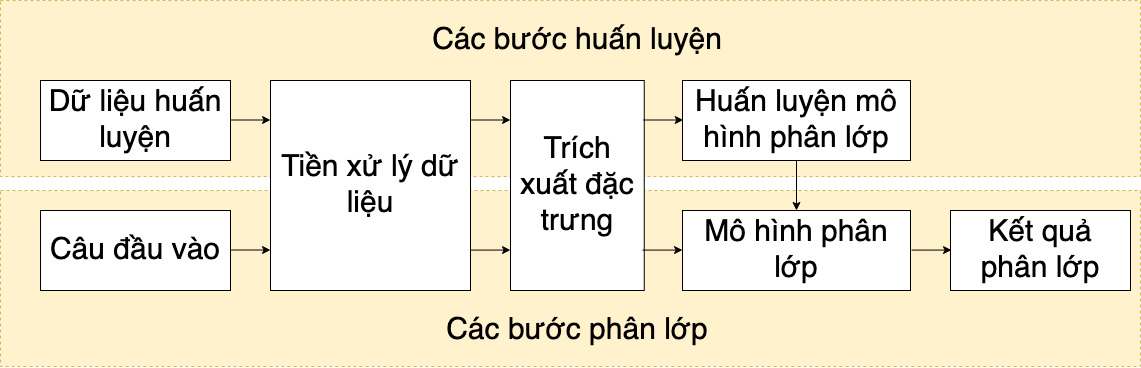
\includegraphics[width=10cm]{images/structure-system-class-intent.png}
    \caption{Kiến trúc của hệ thống phân lớp intent}
    \label{fig:system-class-intent}
\end{figure}

Hệ thống phân lớp intent có một số thành phần cơ bản:
\begin{itemize}
    \item[--] Tiền xử lý dữ liệu
    \item[--] Trích xuất đặc trưng
    \item[--] Huấn luyện mô hình
    \item[--] Phân lớp
\end{itemize}
Trong bước tiền xử lý dữ liệu, chúng ta sẽ thực hiện các thao tác “làm sạch” dữ liệu như: loại bỏ các thông tin dư thừa, chuẩn hoá dữ liệu như chuyển các từ viết sai chính tả thành đúng chính tả, chuẩn hoá các từ viết tắt,… Việc tiền xử lý dữ liệu có vai trò quan trọng trong hệ thống chatbot do đặc thù của ngôn ngữ chat, nói: viết tắt, sai chính tả, hay dùng “teencode”.

Sau khi tiền xử lý dữ liệu và thu được dữ liệu đã được làm sạch, chúng ta sẽ trích xuất những đặc trưng từ dữ liệu này. Trong học máy, bước này được gọi là trích xuất đặc trưng (feature extraction hay feature engineering). Trong mô hình học máy truyền thống (trước khi mô hình học sâu được áp dụng rộng rãi), bước trích xuất đặc trưng ảnh hưởng lớn đến độ chính xác của mô hình phân lớp. Để trích xuất được những đặc trưng tốt, chúng ta cần phân tích dữ liệu khá tỉ mỉ và cần cả những tri thức chuyên gia trong từng miền ứng dụng cụ thể.

Bước huấn luyện mô hình nhận đầu vào là các đặc trưng đã được trích xuất và áp dụng các thuật toán học máy để học ra một mô hình phân lớp. Các mô hình phân lớp có thể là các luật phân lớp (nếu sử dụng decision tree) hoặc là các vector trọng số tương ứng với các đặc trưng được trích xuất (như trong các mô hình logistic regression, SVM, hay mạng Neural).

Sau khi có một mô hình phân lớp intent, chúng ta có thể sử dụng nó để phân lớp một câu hội thoại mới. Câu hội thoại này cũng đi qua các bước tiền xử lý và trích xuất đặc trưng, sau đó mô hình phân lớp sẽ xác định “điểm số” cho từng intent trong tập các intent và đưa ra intent có điểm cao nhất.

\section{Trích xuất thông tin}

Cách tiếp cận phổ biến cho bài toán trích xuất thông tin là mô hình hoá bài toán thành bài toán gán nhãn chuỗi (sequence labeling). Đầu vào của bài toán gán nhãn chuỗi là một dãy các từ, và đầu ra là một dãy các nhãn tương ứng các các từ trong đầu vào. Chúng ta sẽ sử dụng các mô hình học máy để học một mô hình gán nhãn từ một tập dữ liệu đầu vào bao gồm các cặp (x1…xn, y1…yn), trong đó x1…xn là dãy các từ, y1…yn là dãy các nhãn. Độ dài của các dãy từ trong tập dữ liệu có thể khác nhau.

Trong bài toán trích xuất thông tin, tập nhãn cho các từ trong câu đầu vào thường được tạo ra theo  mô hình BIO, với B là viết tắt của “Beginning”, I là viết tắt của “Inside”, và O là viết tắt của “Outside”. Khi biết vị trí từ bắt đầu của một thực thể và các từ nằm trong thực thể đó, chúng ta có thể xác định vị trí của thực thể trong câu. Trong ví dụ ở trên, dãy các nhãn tương ứng với dãy của các từ trong câu hội thoại đầu vào được minh hoạ ở hình \ref{fig:model-BIO}.

Thuật toán huấn luyện mô hình gán nhãn chuỗi phổ biến là mô hình Markov ẩn (HMM – Hidden Markov Models) \cite{2}, mô hình CRF (Conditional Random Fields) \cite{3}. Với dữ liệu văn bản, mô hình CRF thường cho kết quả tốt hơn mô hình HMM. Có khá nhiều các công cụ mã nguồn mở cài đặt mô hình CRF cho bài toán gán nhãn chuỗi như CRF++ \cite{4}, CRF Suite \cite{5}, Mallet \cite{6},…

\begin{figure}[htp]
    \centering
    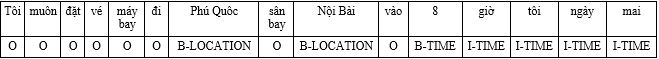
\includegraphics[width=10cm]{images/Model-BIO.png}
    \caption{Gán nhãn từ theo mô hình B-I-O trong trích xuất thông tin}
    \label{fig:model-BIO}
\end{figure}

\section{Giải pháp xây dựng ứng dụng}
Dưới đây là sơ đồ xây dựng ứng dụng chatbot:
\begin{figure}[htp]
    \centering
    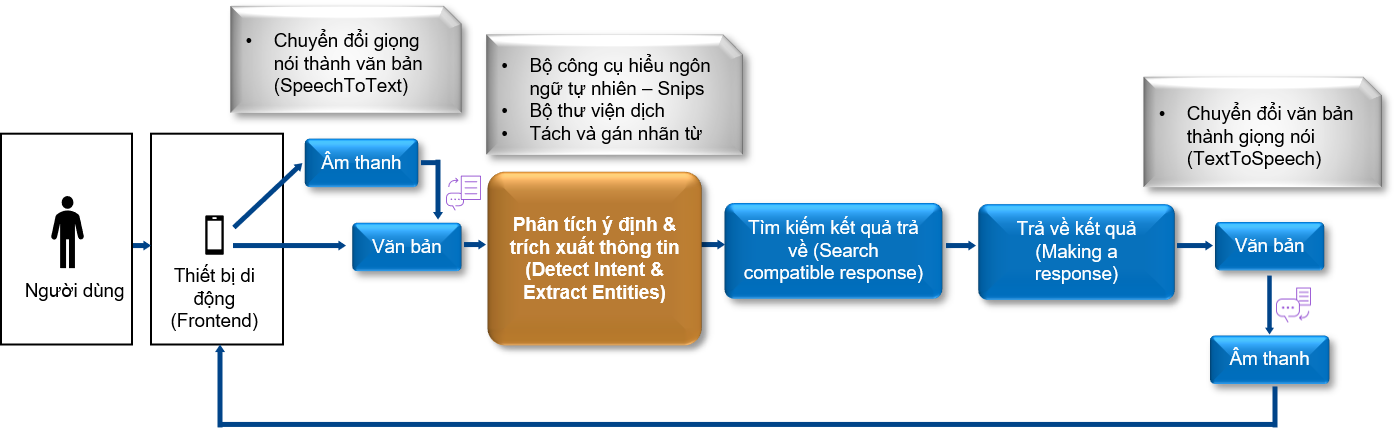
\includegraphics[width=10cm]{images/Structure-description.png}
    \caption{Sơ đồ của hệ thống chỉ đường}
    \label{fig:sodohethongchiduong}

\end{figure}

Sơ đồ này thể hiện các bước thực hiện để xây dựng ứng dụng chatbot từ dữ liêụ đầu vào đến kết quả nhận được. Các bước thực hiện được triển khai như sau:
\begin{itemize}
    \item[--] Bước 1: Khi người dùng sử dụng ứng dụng di động gửi một câu truy vấn bằng audio thì ứng dụng di động sẽ chuyển giọng nói đó thành văn bản (speech to text).
    \item[--] Bước 2: Văn bản đó được gửi tới NLU engine để trích xuất ý định và các thực thể.
    \item[--] Bước 3: Dựa trên ý định và thực thể nhận được, hệ thống sẽ tìm kiếm câu trả lời tương ứng và trả về cho người dùng bằng text và audio (text to speech để chuyển văn bản thành giọng nói).
\end{itemize}
Trong phạm vi đề tài, nhóm sẽ xây dựng thành phần xác định ý định,trích xuất dữ liệu và tìm kiếm kết quả trả lời câu hỏi sẽ sử dụng API của Google Map.

Nhóm chúng em quyết định sử dụng Snips \ac{nlu} cho việc xác định intent vì:
\begin{itemize}
    \item[--] Miễn phí vì nó là opensource
    \item[--] Gọn nhẹ và dễ dàng sử dụng vì có cộng đồng lớn
    \item[--] Hiệu suất cao.
\end{itemize}

Trong hình dưới đây(Xem hình Bảng so sánh \ref{fig:benchmarks}), điểm F1 của cả phân loại ý định và trích xuất slot đã được tính toán cho một số nhà cung cấp NLU và được tính trung bình trên ba bộ dữ liệu Lights dataset\footnote{Xem thêm về Lights dataset tại đây:\url{https://github.com/snipsco/snips-nlu/blob/master/sample_datasets/lights_dataset.json}}, Beverage dataset\footnote{Xem thêm về Beverage dataset tại đây:\url{https://github.com/snipsco/snips-nlu/blob/master/sample_datasets/beverage_dataset.json}}, Flights dataset\footnote{Xem thêm về Flights dataset tại đây:\url{https://github.com/snipsco/snips-nlu/blob/master/sample_datasets/flights_dataset.json}}.

\begin{figure}[htp]
    \centering
    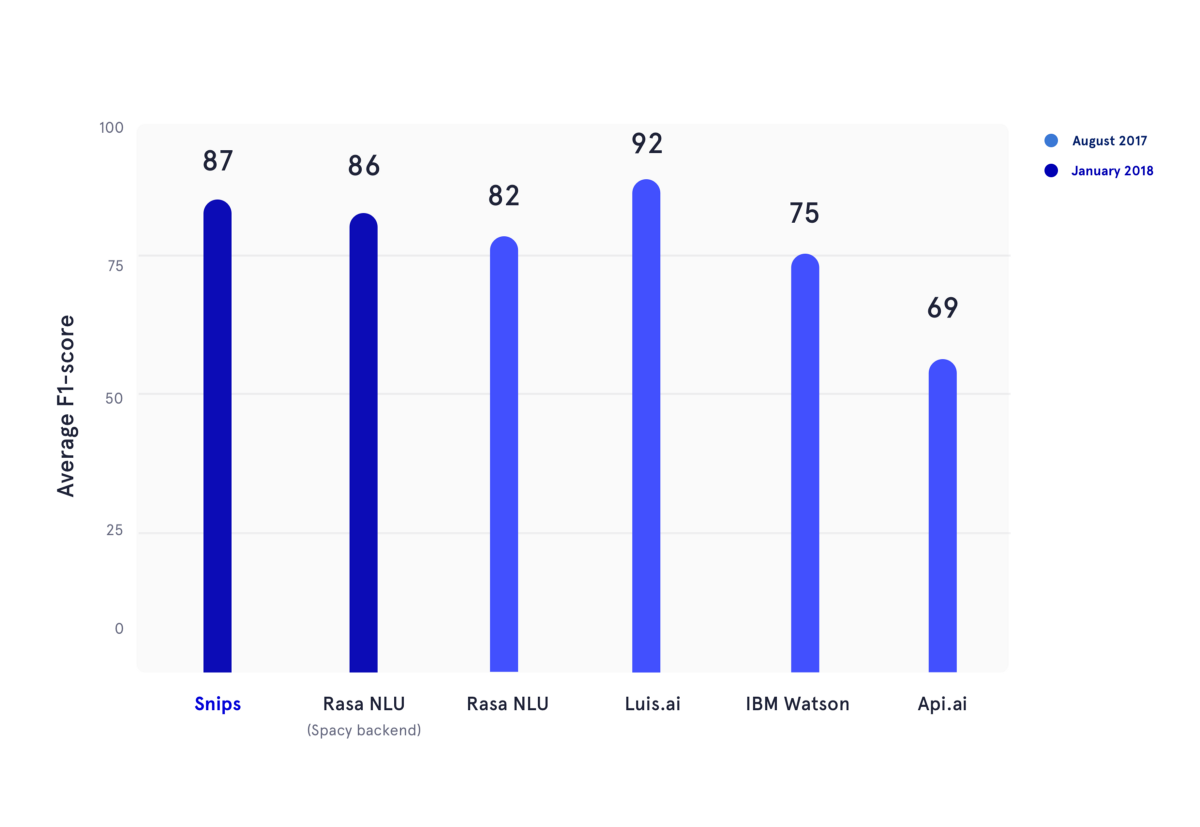
\includegraphics[width=10cm]{images/benchmarks.png}
    \caption{Bảng so sánh}
    \label{fig:benchmarks}
\end{figure}

Snips NLU là công cụ giúp hiểu ngôn ngữ tự nhiên mạnh mẽ, nhưng hiện tại chưa hỗ trợ tiếng Việt, mục tiêu của chúng em là xây dựng một chatbot bằng tiếng Việt. Vì thế, để có thể sử dụng được Snips-nlu để trích xuất ý định và thực thể, chúng em tiến hành thực hiện các bước sau đây:
\begin{itemize}
    \item[--] Bước 1: Tạo một bộ dữ liệu bằng tiếng Việt với các câu nói về chủ đề đường đi.
    \item[--] Bước 2: Chuyển hoá dữ liệu tiếng Việt sang tiếng Anh.
    \item[--] Bước 3: Dùng dữ liệu tiếng Anh được dịch sang để huấn luyện cho mô hình.
    \item[--] Bước 4: Chuyển hoá văn bản bằng tiếng Việt nhận vào sang tiếng Anh.
    \item[--] Bước 5: Đưa câu nói bằng tiếng Anh vào mô hình để trích xuất ý định và các thực thể.
\end{itemize}

Về mặt dữ liệu:
\begin{itemize}
    \item[--] Định dạng bộ dữ liệu huấn luyện là ở dạng json.
\end{itemize}

\section{Chuyển hoá dữ liệu tiếng Việt sang tiếng Anh}
\subsection{Tiền xử lý dữ liệu}


\subsection{Word2word}

Đầu tiên, chúng em dịch bộ dữ liệu từng từ bằng cách tách 1 câu thành từng từ rồi sử dụng thư viện (word2word) để dịch sang tiếng Anh.Vd để dịch câu: "cách đi từ đại học Kinh Tế đến đại học Văn Lang".
\begin{itemize}
    \item[--] Tách câu thành từng từ riêng biệt: ['cách', 'đi', 'từ', 'đại', 'học', 'Kinh' ,'Tế' ,'đến', 'đại', 'học', 'Văn', 'Lang']
    \item[--] Dịch từng từ sang tiếng Anh, ta được: ['ways', 'gone', 'word', 'Swordsman', 'learn', 'GrosDs', 'Monk', 'until', 'Swordsman', 'learn', 'Lam', 'Lang']
\end{itemize}

Sau khi dịch ta được bộ dữ liệu huấn luyện\footnote{Xem thêm về bộ huấn luyện \url{https://drive.google.com/file/d/1nfwUaNtGlk2c5oeK8b6v0lFKC2sb4uAa/view?usp=sharing}} và bộ dữ liệu kiểm thử\footnote{Xem thêm về bộ kiểm thử \url{https://drive.google.com/file/d/1Lo7Ec5CCPmH0nk3vz1LKXO1iZ2dDP9p1/view?usp=sharing}}
\begin{figure}[htp]
    \centering
    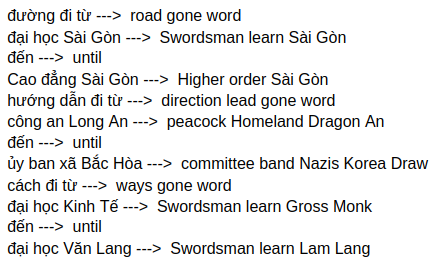
\includegraphics[width=10cm]{images/trainingdata_dichtungtu.png}
    \caption{Hình ảnh minh họa dữ liệu trước khi dịch và sau khi dịch}
    \label{fig:trainingdata_dichtungtu}
\end{figure}

Đem bộ dữ liệu để huấn luyện và đánh giá, ta đạt được kết quả như \ref{fig:metrics-word2word}), xem chi tiết \footnote{\url{https://drive.google.com/file/d/15smz_5u4nV2Wy3yGMAemE8fbdjXFMiPZ/view?usp=sharing}}:

\begin{figure}[htp]
    \centering
    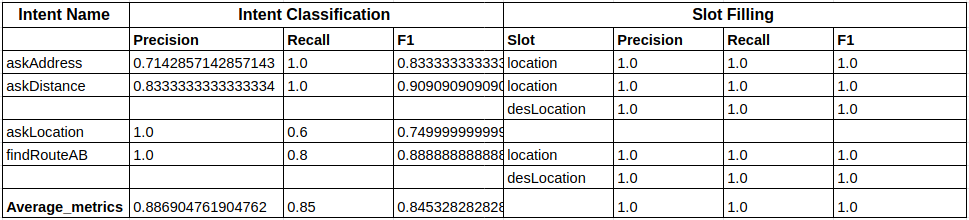
\includegraphics[width=15cm]{images/metrics-word2word.png}
    \caption{Các chỉ số của mô hình}
    \label{fig:metrics-word2word}
\end{figure}
Nhận xét kết quả đạt được:
\begin{itemize}
    \item[--] Mặc dù kết quả tương đối tốt nhưng phương pháp dịch từng từ này không khả thi bởi vì sẽ mà mất ý nghĩa của câu nói, ví dụ như câu sau: "từ Đại học Khoa học Tự nhiên đến Đại học Bách khoa đi như thế nào" được dịch thành "word Swordsman learn department learn itself course until Swordsman learn centurion department" Các thực thể địa điểm như "Đại học Khoa học Tự nhiên" được dịch thành "Swordsman learn department learn itself course", "Đại học Bách khoa" dịch thành "Swordsman learn centurion department"
    \item[--] Các thực thể cần được trích xuất đã bị dịch ra và không còn ý nghĩa nữa, không thể dùng để tìm kiếm địa điểm này trên Google map được.
\end{itemize}
\subsection{Kết hợp word segmentation, pos tagging với word2word}

Nhận thấy được vấn đề về các từ ghép và tên riêng sau khi dịch bằng phương pháp word2word không được chính xác và đúng ý nghĩa của câu. Chúng em tiến hành xem xét về vấn đề phân tách các từ.

Tách từ là một quát trình xử lý nhằm mục đích xác định ranh giới của các từ trong câu văn, cũng có thể hiểu đơn giản hơn là tách từ là quá trình xác định các từ đơn, từ ghép, danh từ,... có trong câu.

Để xử lý vấn đề dịch các tên riêng và không đúng ngữ nghĩa, nhóm em thay đổi phương pháp dịch bằng cách sử dụng thư viện để tách từ (word segmentation) và gán nhãn từ loại (pos tagging).

Trong tiếng Việt, dấu cách (space) không được sử dụng như 1 kí hiệu phân tách từ, nó chỉ có ý nghĩa phân tách các âm tiết với nhau. Do đó việc tách từ sẽ giúp cho việc dịch được chính xác hơn.

Về vấn đề những slot bị dịch thành tiếng Anh làm cho nó không còn ý nghĩa nữa, nhóm em nhận thấy rằng những slot này chủ yếu là danh từ, nên nhóm sẽ sử dụng pos tagging để gán nhãn từ loại, những từ nào thuộc danh từ thì sẽ không cho dịch thành tiếng Anh.

Áp dụng word segmentation và pos tagging lên bộ dữ liệu và sử dụng thư viện word2word để dịch thì đạt được bộ dữ liệu huấn luyện\footnote{Xem thêm về bộ huấn luyện \url{https://drive.google.com/file/d/1KE6IMt7KTVu5LRQWI9b57EUgWuqBRgp_/view?usp=sharing}} và bộ dữ liệu kiểm thử\footnote{Xem thêm về bộ kiểm thử\url{https://drive.google.com/file/d/1YHs3dFAT0br8RbctmWYQtdIKQmv6j1su/view?usp=sharing}}:

\begin{figure}[htp]
    \centering
    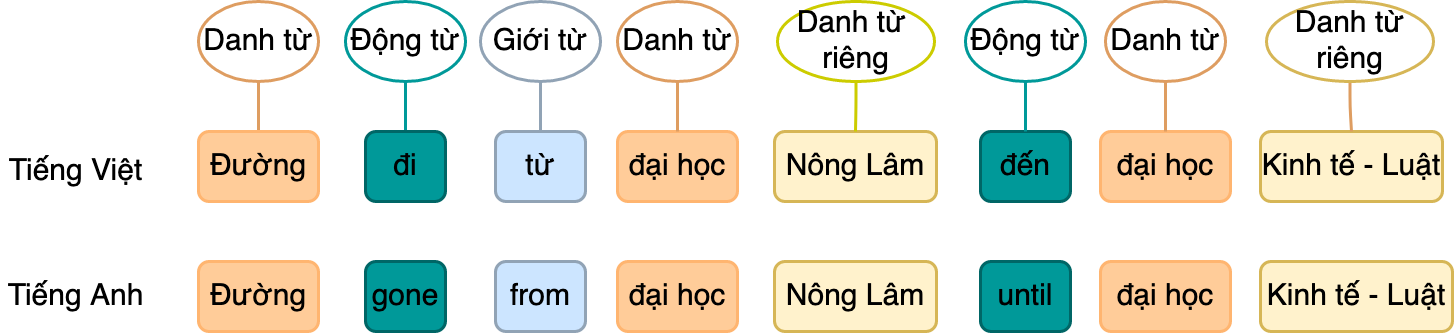
\includegraphics[width=10cm]{images/trainingdata-wordsegment.png}
    \caption{Hình ảnh minh họa dữ liệu trước khi dịch và sau khi dịch bằng phương pháp dùng word segmentation và pos tagging}
    \label{fig:trainingdata-wordsegment}
\end{figure}

Sau khi huấn luyện mô hình và đem đi đánh giá nhóm nhận được kết quả như \ref{fig:metrics-word2word-postag}, xem chi tiết \footnote{\url{https://drive.google.com/file/d/1pBegsfVWfMpW-YQHFQvhh1mX49uOESLF/view?usp=sharing}}:

\begin{figure}[htp]
    \centering
    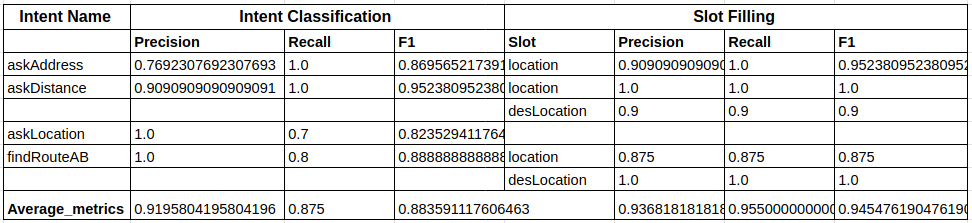
\includegraphics[width=15cm]{images/metrics-word2word+postag.png}
    \caption{Các chỉ số của mô hình}
    \label{fig:metrics-word2word-postag}
\end{figure}

Nhận xét kết quả đạt được:
\begin{itemize}
    \item[--] Sau khi áp dụng tách từ và phân loại từ vựng, nhóm đã xử lý tương đối được vấn đề dịch những slot làm mất ý nghĩa của chúng: "từ Đại học Khoa học Tự nhiên đến Đại học Bách khoa đi như thế nào" được dịch thành "word đại\_học khoa\_học\_tự\_nhiên until đại\_học bách\_khoa gone như\_thế\_nào"
\end{itemize}
Tuy nhiên vẫn còn một vài trường hợp dịch còn chưa ổn, ví dụ:
\begin{itemize}
    \item[--] "Đại học Khoa học Xã hội và Nhân văn" được dịch thành "Đại học Khoa học Xã hội their Nhân văn".
    \item[--] Một số từ được dịch không đúng ngữ cảnh. Ví dụ như: "từ" => "word"; "đến" => "until".
\end{itemize}


\subsection{Xây dựng bộ từ điển}
Để có thể xử lý tốt hơn về vấn đề ý nghĩa trong câu được dịch sang một cách chính xác hơn. Nhóm chúng em đã quyết định xây dựng mô hình so khớp dài nhất (longest matching), bằng cách xây dựng một bộ từ điển, và tìm từ dài nhất có trong bộ từ điển đó để tiến hành dịch. Bộ từ điển này nằm trong phạm vi hỏi đường nên có thể xây dựng với các từ ngữ cụ thể có trong chủ đề, từ đó việc dịch sẽ đạt hiệu quả hơn.

Trong phạm vi các câu hỏi về đường đi, chúng em đã lựa chọn dịch khoảng 50 từ và các cụm từ. Các bước để dịch được dữ liệu như sau:
\begin{itemize}
    \item[--] Bước 1: Xây dựng bộ từ điển riêng biệt về chủ đề hỏi đường đi và chuyển hoá từ ngôn ngữ tiếng Việt sang tiếng Anh.
    \item[--] Bước 2: Tìm từ dài nhất trong câu có trong bộ từ điển.
    \item[--] Bước 3: Lấy nghĩa của từ tương ứng trong từ điển.
\end{itemize}
Trong quá trình nghiên cứu, chúng em nhận thấy bước 2 là bước thật sự cần thiết để có thể tìm được từ thích hợp nhất với bộ từ điển để có kết quả tốt nhất. Dưới đây là mô tả quá trình tìm từ dài nhất có trong từ điển mà nhóm chúng em thực hiện (Xem hình Tìm từ dài nhất \ref{fig:longest-word})
\begin{itemize}
    \item[--] Input: "Đường đi từ Đại học Nông Lâm đến Ngã tư Thủ Đức""
    \item[--] Output: ["Đường đi", "từ", "Đại học Nông Lâm", "đến", "Ngã tư Thủ Đức"]
\end{itemize}
\begin{figure}[htp]
    \centering
    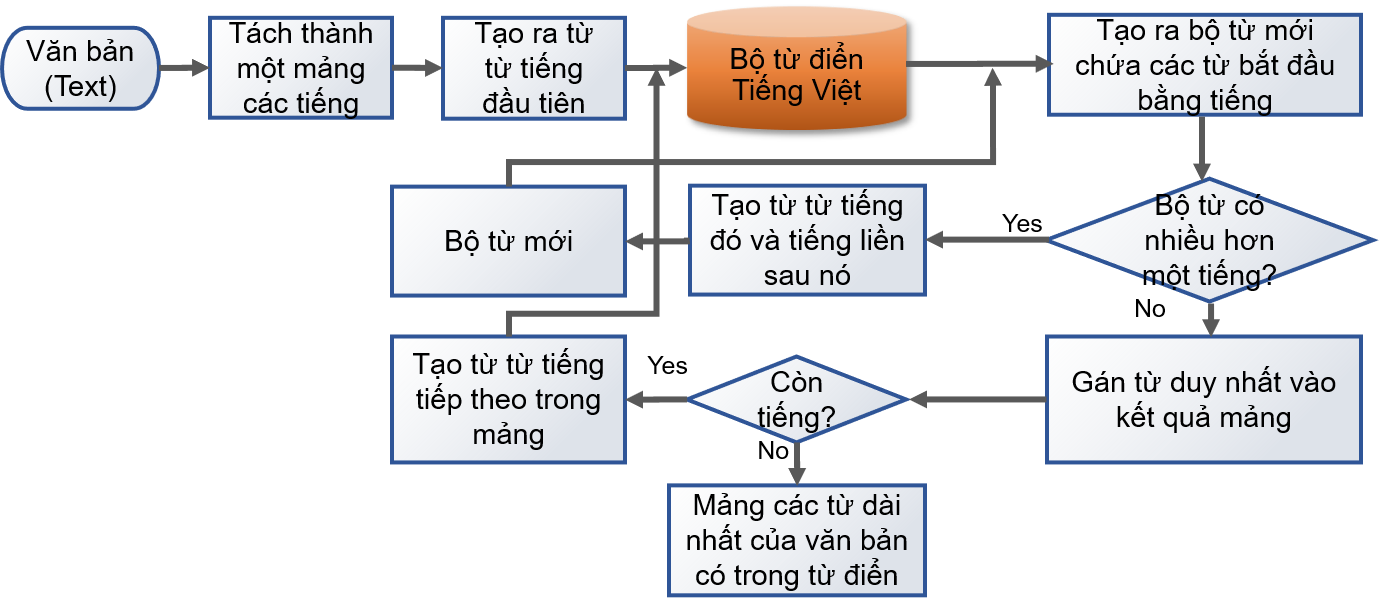
\includegraphics[width=10cm]{images/Diagram-longest-word.png}
    \caption{Tìm từ dài nhất}
    \label{fig:longest-word}
\end{figure}

Sau khi dịch ta được bộ dữ liệu huấn luyện\footnote{Xem thêm về bộ huấn luyện \url{https://drive.google.com/file/d/1VSDhjrSghKtHmQxhWfC_x-qyOKDm3YuM/view?usp=sharing}} và bộ dữ liệu kiểm thử \footnote{Xem thêm về bộ kiểm thử \url{https://drive.google.com/file/d/1S631oRroP67z6LRwGSNwkrx-22c10baJ/view?usp=sharing}}
\begin{figure}[htp]
    \centering
    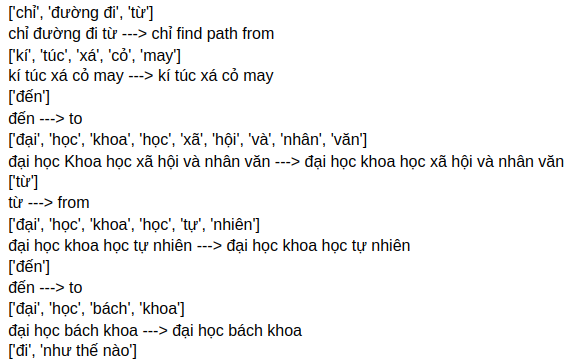
\includegraphics[width=10cm]{images/trainingdata-tudien.png}
    \caption{Hình ảnh minh họa dữ liệu trước khi dịch và sau khi dịch bằng phương pháp xây dựng từ điển}
    \label{fig:trainingdata-tudien}

\end{figure}

Đem bộ dữ liệu để huấn luyện và đánh giá, ta đạt được kết quả như \ref{fig:metrics-dict-ex}, xem chi tiết \footnote{\url{https://drive.google.com/file/d/1EGU3twPZBkS-zSkmIJ8viifMRkOXstvV/view?usp=sharing}}:

\begin{figure}[htp]
    \centering
    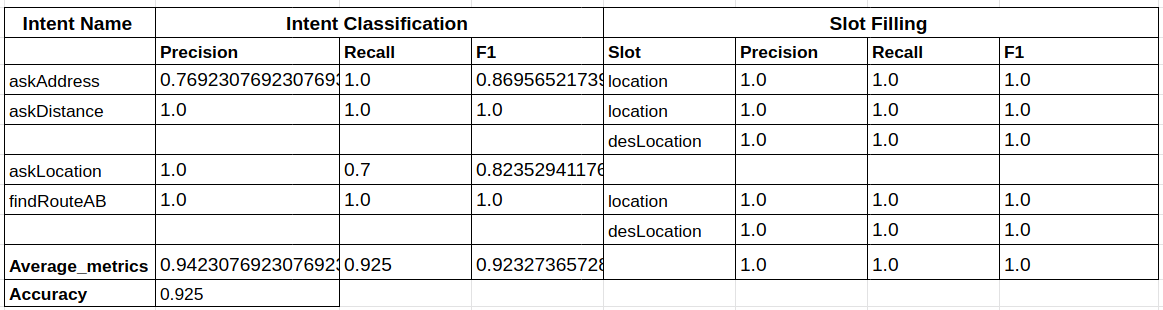
\includegraphics[width=15cm]{images/metrics-dict}
    \caption{Các chỉ số của mô hình}
    \label{fig:metrics-dict-ex}
\end{figure}
Kết quả đạt được sau khi dùng phương pháp dịch bằng cách xây dựng bộ từ điển:
\begin{itemize}
    \item[--] Do xây dựng bộ từ điển những từ vựng trong phạm vi nhỏ - hỏi đường nên bộ dịch cho ra kết quả khá khả quan, cải thiện hơn so với 2 phương pháp trước là phương pháp dịch từng từ và phương pháp dịch dùng word segmentation và pos tagging
\end{itemize}

\section{Công nghệ}

\subsection{Flutter}
Để xây dựng giao diện web cho hệ thống nhóm đã tiến hành tìm hiểu nhiều công nghệ xây dựng mobile như React Native\footnote{Xem thêm về React Native tại đây: \url{https://reactnative.dev/}}, Xamarin\footnote{Xem thêm về Xamarin tại đây: \url{https://docs.microsoft.com/en-us/xamarin/}}, Flutter\footnote{Flutter là một bộ công cụ giao diện người dùng để xây dựng ứng dụng cho nhiều nền tảng khác nhau như web, thiết bị di động, máy tính cá nhân với cùng một mã nguồn. Xem thêm về Flutter tại đây: \url{https://flutter.dev/}}.

Nhóm quyết định chọn Flutter vì các ưu điểm sau:
\begin{itemize}
    \item[--] Flutter là công nghệ mới nhưng có cộng đồng sử dụng đông đảo và phát triển nhanh, dễ dàng tìm được hỗ trợ nếu xảy ra lỗi
    \item[--] Bộ giao diện dựng sẵn của Flutter tuân thủ đầy đủ bộ quy tắc thiết kế giao diện Material Design\footnote{Bộ quy tắc thiết kế giao diện hiện đại và phổ biến của Google. Xem thêm về Material Design tại đây: \url{https://material.io/design}}, mang đến một giao diện hiện đại cho hệ thống
    \item[--] Flutter mang đến tính năng hot reload\footnote{Tính năng cho phép những thay đổi trong mã nguồn được hiển thị gần như lập tức trên giao diện}, kết hợp với bộ giao diện dựng sẵn và trình kiểm tra lỗi dễ sử dụng giúp quá trình phát triển nhanh chóng
\end{itemize}

\subsection{Snips NLU}
Snips-NLU - bộ công cụ trích xuất thông tin có cấu trúc từ các câu được viết bằng ngôn ngữ tự nhiên mã nguồn mở được viết bằng Python.
Đây là một bộ công cụ được sử dụng rộng rãi để phục vụ những nhà nghiên cứu hiểu ngôn ngữ tự nhiên - NLU (Natural Language Understanding) nhằm xây dựng một hệ thống hiểu được ngôn ngữ mà con người sử dụng. Các bài báo liên quan mà nhóm tìm hiểu được sử dụng trong đề tài được thực hiện trên bộ công cụ này. Mô hình huấn luyện được nhóm tự xây dựng và sử dụng công cụ này để huấn luyện.

\subsection{Flask Python}
Python ngày càng chứng minh ưu thế của mình trong việc xây dựng và triển khai nhiều loại ứng dụng khác nhau như web application, desktop application, Machine Leaning, Deep Learning….
Để xây dựng \ac{api} cho hệ thống và thuận tiện cho việc nghiên cứu, nhóm chúng em đã tiến hành tìm hiểu nhiều framwork để xây dựng trên Python như Flask\footnote{Xem thêm về Flask tại đây:\url{https://flask.palletsprojects.com}}, Django\footnote{Xem thêm về Django tại đây:\url{https://docs.djangoproject.com}}, Tornado \footnote{Xem thêm về Tornado tại đây: \url{https://www.tornadoweb.org}}, Pyramid\footnote{Xem thêm về Pyrmaid tại đây: \url{https://docs.pylonsproject.org/}}

Nhóm quyết định chọn Flask Python vì các ưu điểm sau:
\begin{itemize}
    \item[--] Đơn giản và dễ dàng sử dụng
    \item[--] Flask Python là micro web framework, không cần công cụ hoặc thư viện cụ thể, nó mang đến các chức năng tối giản nhưng có thể mở rộng cho các ứng dụng web.
    \item[--] Hỗ trợ xây dựng các API, web services, các ứng dụng web application cỡ vừa và nhỏ.
    \item[--] Flask cung cấp rất nhiều tài liệu từ cài đặt đến thực hiện và triển khai, từ hướng dẫn nhanh đến hướng dẫn chi tiết. Nguồn tài liệu tham khảo về Flask rất phong phú giúp dễ dàng tham khảo và tìm hiểu.
\end{itemize}

Theo đánh giá năm 2020 của JetBrains Python Developers Survey\footnote{Xem thêm tại đây: \url{https://www.jetbrains.com/lp/python-developers-survey-2020/}} thì Flask hiện là framework được sử dụng rộng rãi nhất, chiếm tới 46\% thị phần.
\subsection{Google Maps API}
Google Maps API \footnote{Xem thêm về React Native tại đây: \url{https://developers.google.com/maps/documentation}} là một phương pháp cho phép một website, ứng dụng B có thể sử dụng dịch vụ hoặc hiển thị nội dung của một trang web khác, ở đây là website A – Google Maps (thông qua Map API), dịch vụ bản đồ của website A (Map) sẽ được nhúng vào website B (Website cá nhân), tại trang web B có thể sử dụng những dịch vụ mà Google Maps cung cấp thông qua Google Maps API như: đường đi, đánh dấu trên bản đồ, danh sách các địa điểm muốn tìm,...

Hiện nay, các ứng dụng xây dựng trên nền tảng Google Maps như Grab, AndroidAuto,... thường sử dụng Google Maps API để nhúng bản đồ vào trang web hoặc ứng dụng thông qua nhiều cách khác nhau, chính vì vậy mà việc sử dụng API từ Google cũng khá dễ dàng. Đồng thời Map API cũng không chỉ hỗ trợ cho máy tính và website mà còn cả thiết bị di động, giúp ứng dụng hoạt động nhanh hơn và hiệu quả hơn.

Một số ứng dụng của Google Maps API :
\begin{itemize}
    \item[–-] Tính năng chỉ đường đến địa điểm cần tìm (tuyến đường tối ưu nhất cho các phương tiện và nhiều lựa chọn khác).
    \item[–-] Giúp khoanh vùng khu vực như khu đô thị hay các khu vực mà bạn muốn.
    \item[–-] Có thể theo dõi tình hình giao thông, lưu lượng phương tiện tại các khu vực,... và có giải pháp hợp lý.
\end{itemize}
